% !TEX encoding = UTF-8 Unicode
\documentclass[12pt,a4paper]{article}

\usepackage[utf8]{inputenc}
\usepackage[T1]{fontenc}
\usepackage[polish]{babel}
\usepackage{geometry}
\usepackage{booktabs}
\usepackage{longtable}
\usepackage{listings}
\usepackage{xcolor}
\usepackage{graphicx}
% Fallback dla grafik: dziala zarowno przy kompilacji z katalogu docs/,
% jak i z katalogu glownego repozytorium (pdflatex docs/dokumentacja.tex).
\graphicspath{{./}{docs/}{psbd/erd/}{docs/psbd/erd/}}
\usepackage{parskip}
\usepackage{titlesec}
\usepackage{array}
\usepackage{caption}
\usepackage{enumitem}
\usepackage{fancyhdr}
\usepackage{lmodern}
\usepackage{amssymb}
% hyperref ladowany na koncu preambury, zeby uniknac konfliktow z innymi pakietami
\usepackage{hyperref}

\geometry{
  top=2.5cm,
  bottom=2.5cm,
  left=2.5cm,
  right=2.5cm
}

% --- Kolory i styl listings ---
\definecolor{codebg}{RGB}{248,248,248}
\definecolor{codeframe}{RGB}{200,200,200}
\definecolor{keywordcolor}{RGB}{0,0,180}
\definecolor{commentcolor}{RGB}{100,100,100}
\definecolor{stringcolor}{RGB}{180,0,0}

\lstdefinestyle{pythonstyle}{
  language=Python,
  backgroundcolor=\color{codebg},
  frame=single,
  rulecolor=\color{codeframe},
  basicstyle=\ttfamily\small,
  keywordstyle=\color{keywordcolor}\bfseries,
  commentstyle=\color{commentcolor}\itshape,
  stringstyle=\color{stringcolor},
  breaklines=true,
  showstringspaces=false,
  tabsize=4,
  numbers=left,
  numberstyle=\tiny\color{gray},
  captionpos=b,
}

\lstdefinestyle{sqlstyle}{
  language=SQL,
  backgroundcolor=\color{codebg},
  frame=single,
  rulecolor=\color{codeframe},
  basicstyle=\ttfamily\small,
  keywordstyle=\color{keywordcolor}\bfseries,
  commentstyle=\color{commentcolor}\itshape,
  stringstyle=\color{stringcolor},
  breaklines=true,
  showstringspaces=false,
  tabsize=2,
  numbers=left,
  numberstyle=\tiny\color{gray},
  captionpos=b,
  morekeywords={EXPLAIN,ANALYZE,RETURNING,SERIAL,BIGSERIAL,BOOLEAN,TEXT,VARCHAR},
}

\lstdefinestyle{yamlstyle}{
  backgroundcolor=\color{codebg},
  frame=single,
  rulecolor=\color{codeframe},
  basicstyle=\ttfamily\small,
  keywordstyle=\color{keywordcolor},
  commentstyle=\color{commentcolor}\itshape,
  stringstyle=\color{stringcolor},
  breaklines=true,
  showstringspaces=false,
  tabsize=2,
  numbers=left,
  numberstyle=\tiny\color{gray},
  captionpos=b,
}

\lstdefinestyle{consolestyle}{
  backgroundcolor=\color{codebg},
  frame=single,
  rulecolor=\color{codeframe},
  basicstyle=\ttfamily\small,
  breaklines=true,
  captionpos=b,
}

% --- Nagłówek/stopka ---
\pagestyle{fancy}
\fancyhf{}
\rhead{U Alchemika System -- Dokumentacja techniczna}
\lhead{}
\cfoot{\thepage}

% --- Hyperref ---
\hypersetup{
  colorlinks=true,
  linkcolor=blue,
  urlcolor=blue,
  citecolor=blue,
  pdftitle={U Alchemika System -- Dokumentacja bazy danych},
  pdfauthor={Maciej Bulhak},
}

% ---------------------------------------------------------------
\begin{document}

% ===================== STRONA TYTUŁOWA =====================
\begin{titlepage}
  \centering
  \vspace*{2cm}
  {\LARGE\bfseries Akademia Techniczno-Humanistyczna \par}
  \vspace{0.5cm}
  {\large Projektowanie systemów baz danych \par}
  \vspace{2.5cm}

  \rule{\linewidth}{0.5mm}
  \vspace{0.6cm}
  {\Huge\bfseries U Alchemika System \par}
  \vspace{0.4cm}
  {\Large System zarządzania agroturystyką \par}
  \vspace{0.4cm}
  {\large\itshape Dokumentacja techniczna bazy danych \par}
  \rule{\linewidth}{0.5mm}

  \vspace{2cm}
  \begin{tabular}{rl}
    \textbf{Autor:}        & Maciej Bulhak \\[4pt]
    \textbf{Data:}         & \today \\[4pt]
    \textbf{Technologia:}  & Django 4.2 + PostgreSQL 16 + Docker \\
  \end{tabular}

  \vfill
  {\small Projekt realizowany w ramach kursu \emph{Projektowanie systemów baz danych} \par}
\end{titlepage}

% ===================== SPIS TREŚCI =====================
\tableofcontents
\newpage

% ===================== 1. CEL I ZAKRES =====================
\section{Cel i zakres projektu}

Celem projektu jest zaprojektowanie, implementacja i~prezentacja systemu bazodanowego
dla obiektu agroturystycznego \textbf{„U Alchemika”} zlokalizowanego w Górach Izerskich
(Jasna Góra, ul.~Górska~3, 59-921). System obsługuje:

\begin{itemize}[nosep]
  \item zarządzanie pokojami i~ich udogodnieniami,
  \item przyjmowanie zapytań rezerwacyjnych od gości,
  \item publikację treści (blog, atrakcje okolicy),
  \item przechowywanie informacji o~obiekcie,
  \item śledzenie działań administracyjnych (log audytu).
\end{itemize}

Projekt realizuje wszystkie etapy cyklu życia systemu bazodanowego: od wyboru SZBD
i~konfiguracji środowiska, przez iteracyjne projektowanie modelu danych, aż po
testowanie i~optymalizację zapytań.

% ===================== 2. ŚRODOWISKO =====================
\section{Wybór środowiska SZBD i konfiguracja deweloperska}

\subsection{Decyzja technologiczna}

Jako system zarządzania bazą danych wybrano \textbf{PostgreSQL~16}. Uzasadnienie:

\begin{itemize}[nosep]
  \item pełna zgodność z~ANSI SQL i~zaawansowane typy danych,
  \item natywna obsługa przez Django ORM (adapter \texttt{psycopg2}),
  \item silne wsparcie dla kluczy obcych i~transakcji ACID,
  \item dostępny oficjalny obraz Docker (\texttt{postgres:16}).
\end{itemize}

Warstwa aplikacyjna to \textbf{Django~4.2} (Python~3.12), który pełni rolę
interfejsu użytkownika (Django Admin) oraz warstwy dostępu do danych (ORM).

\subsection{Infrastruktura Docker}

Środowisko uruchomieniowe zostało skonteneryzowane za pomocą Docker Compose.
Plik \texttt{docker-compose.yml} definiuje dwa serwisy:

\begin{lstlisting}[style=yamlstyle, caption={docker-compose.yml -- konfiguracja serwisów}]
services:
  db:
    image: postgres:16
    container_name: u_alchemika_db
    restart: unless-stopped
    environment:
      POSTGRES_DB: u_alchemika
      POSTGRES_USER: postgres
      POSTGRES_PASSWORD: postgres
    ports:
      - "5432:5432"
    volumes:
      - postgres_data:/var/lib/postgresql/data
    healthcheck:
      test: ["CMD-SHELL", "pg_isready -U postgres -d u_alchemika"]
      interval: 10s
      timeout: 5s
      retries: 5

  web:
    build: ./backend
    container_name: u_alchemika_web
    restart: unless-stopped
    ports:
      - "8000:8000"
    environment:
      POSTGRES_HOST: db
      POSTGRES_PORT: 5432
      POSTGRES_DB: u_alchemika
      POSTGRES_USER: postgres
      POSTGRES_PASSWORD: postgres
      DJANGO_SECRET_KEY: dev-secret-key-not-for-production
      DEBUG: "True"
      DJANGO_ALLOWED_HOSTS: "localhost,127.0.0.1"
    volumes:
      - ./backend:/app
    depends_on:
      db:
        condition: service_healthy

volumes:
  postgres_data:
\end{lstlisting}

\textbf{Sekwencja uruchamiania:}
\begin{enumerate}[nosep]
  \item Kontener \texttt{db} startuje; healthcheck (\texttt{pg\_isready}) czeka
        na gotowość PostgreSQL.
  \item Kontener \texttt{web} buduje obraz i~uruchamia serwer Django dopiero po
        uzyskaniu \texttt{service\_healthy} od \texttt{db}.
  \item Przy starcie Django automatycznie wykonuje \texttt{manage.py migrate},
        a~następnie \texttt{runserver 0.0.0.0:8000}.
\end{enumerate}

Dane PostgreSQL są persystowane w~nazwanym wolumenie \texttt{postgres\_data},
dzięki czemu przeżywają restart kontenerów. Kod aplikacji jest montowany jako
bind-mount (\texttt{./backend:/app}), co umożliwia edycję na żywo bez przebudowy obrazu.

% ===================== 3. ANALIZA WYMAGAŃ =====================
\section{Analiza wymagań i wstępny model danych}

\subsection{Aktorzy systemu}

\begin{description}[nosep]
  \item[Gość] -- osoba odwiedzająca stronę; może przeglądać pokoje i~wysyłać
    zapytanie rezerwacyjne.
  \item[Administrator] -- obsługuje zapytania, zarządza treścią i~danymi obiektu
    poprzez panel Django Admin.
\end{description}

\subsection{Przypadki użycia}

\begin{itemize}[nosep]
  \item Przeglądanie listy pokoi (filtrowanie po aktywnych).
  \item Wyświetlanie szczegółów pokoju (galeria, udogodnienia, cena).
  \item Wysłanie zapytania rezerwacyjnego z~opcjonalnym wskazaniem pokoju i~dat.
  \item Zarządzanie statusem zapytań (nowe / odpowiedziano / zamknięte).
  \item Dodawanie/edytowanie/usuwanie pokoi, udogodnień, postów, atrakcji.
  \item Przeglądanie logu audytu (tylko odczyt).
\end{itemize}

\subsection{Zidentyfikowane encje}

Wstępna analiza wymagań doprowadziła do wyodrębnienia następujących encji
głównych (finalny wykaz opisano w~sekcji~\ref{sec:tabele}):

\begin{center}
\begin{tabular}{lll}
\toprule
\textbf{Encja} & \textbf{Aplikacja} & \textbf{Opis} \\
\midrule
Room & core & Pokój / apartament \\
RoomImage & core & Zdjęcia pokoju \\
Amenity & core & Udogodnienie (WiFi, parking, \ldots) \\
RoomAmenity & core & Relacja N:M Pokój--Udogodnienie \\
Inquiry & core & Zapytanie rezerwacyjne gościa \\
PropertyInfo & core & Dane i~polityki obiektu \\
AuditLog & core & Log działań administratora \\
Post & content & Wpis blogowy \\
Attraction & content & Atrakcja turystyczna \\
\bottomrule
\end{tabular}
\end{center}

\subsection{Diagram ERD}

\begin{figure}[ht]
  \centering
  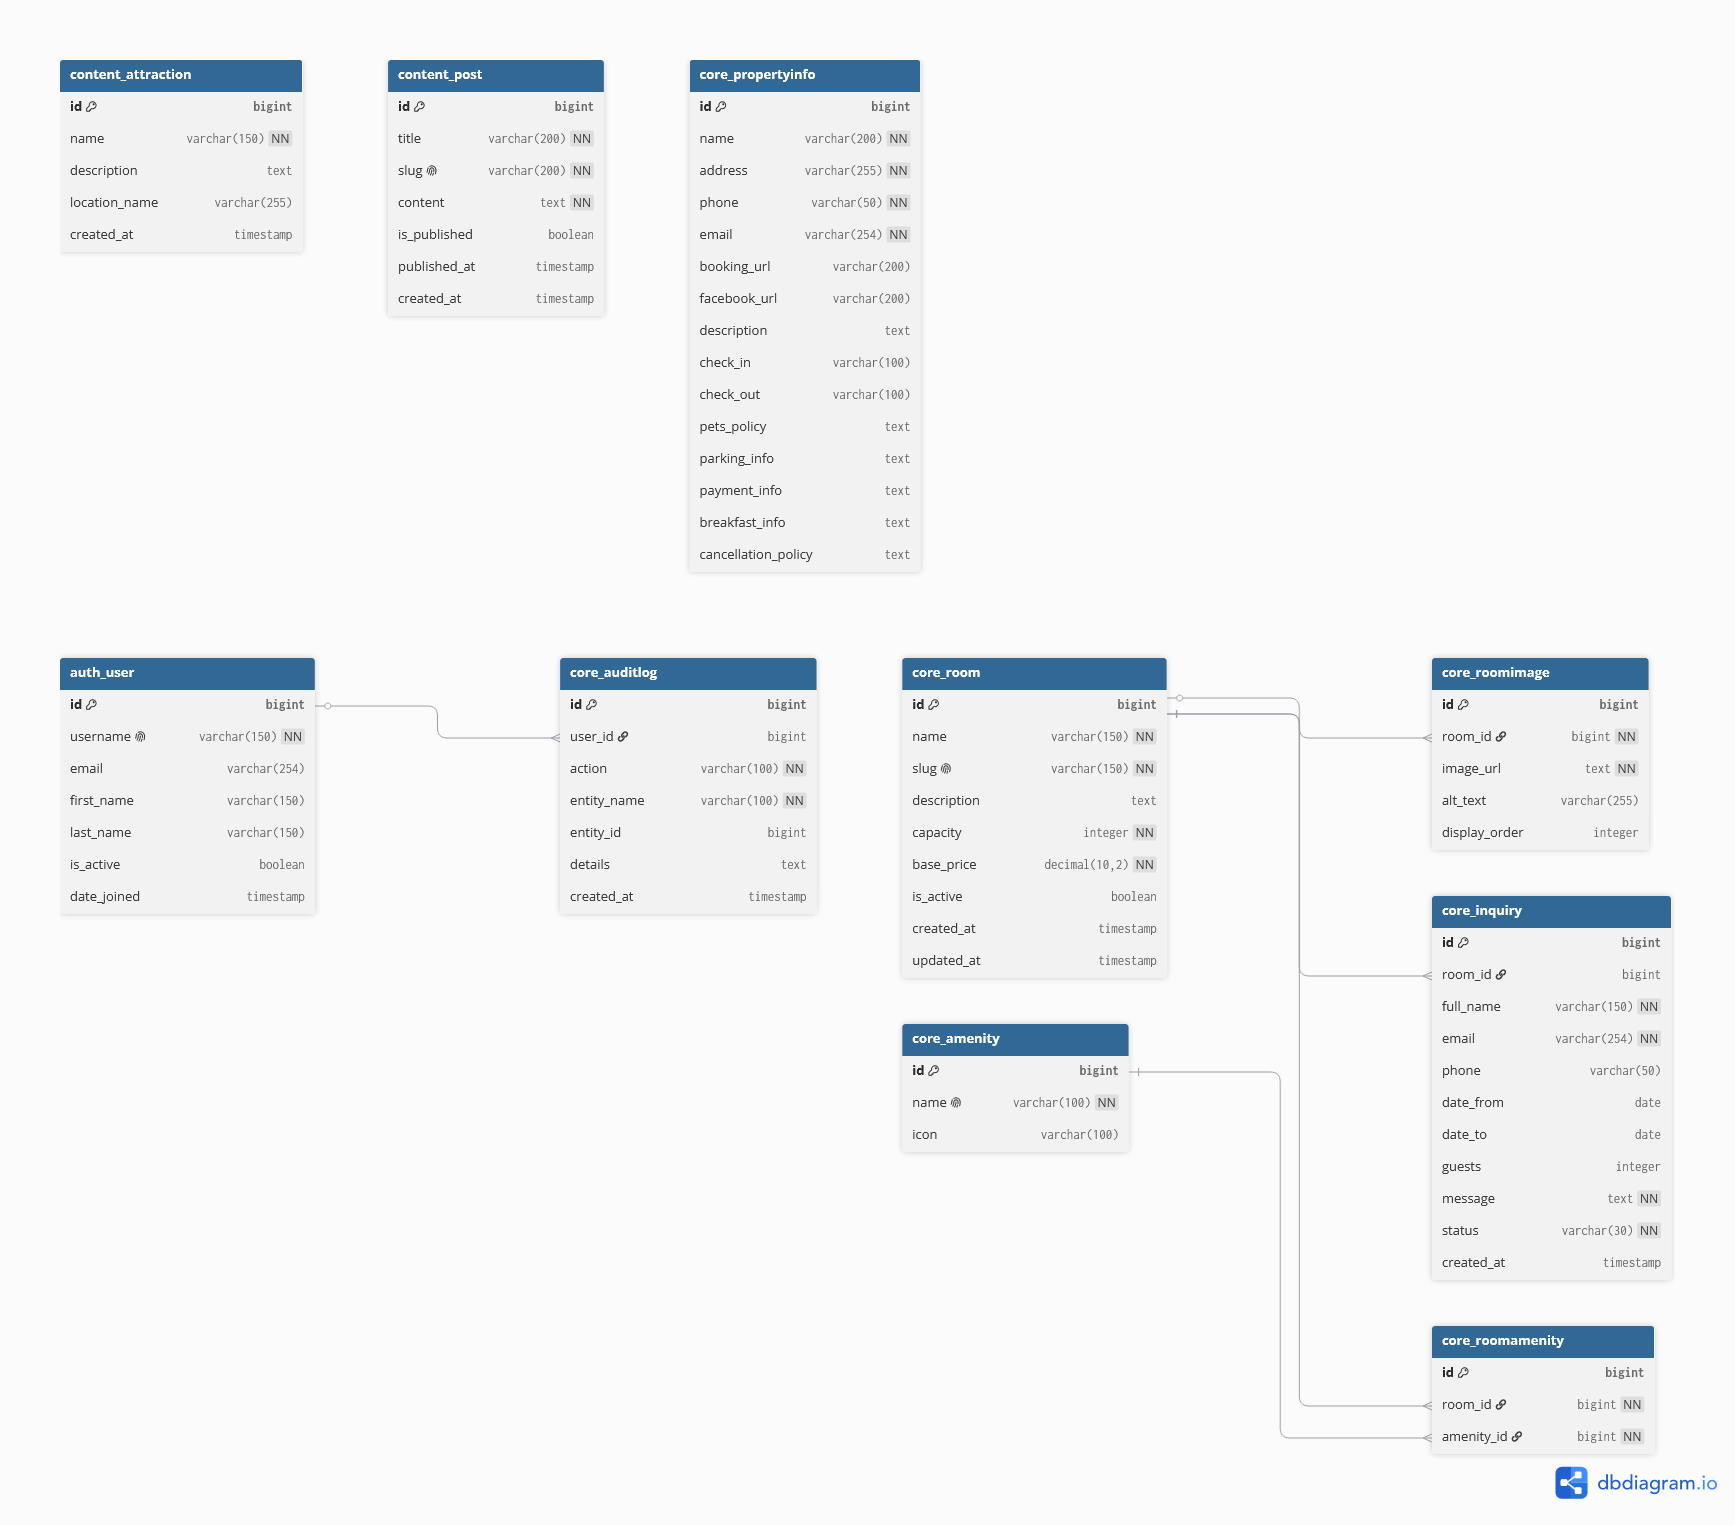
\includegraphics[width=0.95\textwidth]{psbd/erd/erd.png}
  \caption{Diagram encji i~relacji (ERD) systemu U Alchemika}
  \label{fig:erd}
\end{figure}

% ===================== 4. MIGRACJE =====================
\section{Iteracyjne projektowanie -- historia migracji}

System ewoluował poprzez kolejne migracje Django, które stanowią wersjonowany
zapis wszystkich zmian w~strukturze bazy danych.

\subsection{Przegląd migracji}

\begin{longtable}{p{0.25\linewidth}p{0.6\linewidth}}
\toprule
\textbf{Migracja} & \textbf{Zmiany} \\
\midrule
\endfirsthead
\toprule
\textbf{Migracja} & \textbf{Zmiany} \\
\midrule
\endhead
\texttt{core/0001\_initial} &
  Schemat bazowy: tabele \texttt{core\_room}, \texttt{core\_roomimage},
  \texttt{core\_amenity}, \texttt{core\_roomamenity}, \texttt{core\_inquiry},
  \texttt{core\_auditlog}. Indeksy: \texttt{room\_slug\_idx},
  \texttt{inquiry\_status\_idx}, \texttt{inquiry\_email\_idx}. \\[4pt]
\texttt{content/0001\_initial} &
  Tabele treści: \texttt{content\_post}, \texttt{content\_attraction}. \\[4pt]
\texttt{core/0002\_room\_updated\_at} &
  Dodanie kolumny \texttt{updated\_at} (auto-update) do \texttt{core\_room} --
  możliwość śledzenia ostatniej modyfikacji pokoju. \\[4pt]
\texttt{core/0003\_inquiry\_index\_created\_at} &
  Dodanie indeksu \texttt{inquiry\_created\_at\_idx} na \texttt{core\_inquiry.created\_at}
  w~celu optymalizacji sortowania chronologicznego. \\[4pt]
\texttt{core/0004\_propertyinfo} &
  Nowa tabela \texttt{core\_propertyinfo} (14 pól) -- centralne repozytorium
  informacji o~obiekcie i~politykach. \\
\bottomrule
\end{longtable}

\subsection{Rollback migracji}

Każda migracja Django definiuje operację odwrotną. Przykłady cofania:

\begin{lstlisting}[style=consolestyle, caption={Cofanie migracji}]
# Cofniecie do migracji 0001 (usuwa updated_at, indeks i PropertyInfo)
python manage.py migrate core 0001

# Cofniecie calej aplikacji core (usuwa wszystkie tabele core_*)
python manage.py migrate core zero

# Cofniecie aplikacji content
python manage.py migrate content zero
\end{lstlisting}

% ===================== 5. OPIS TABEL =====================
\section{Szczegółowy opis tabel bazy danych}
\label{sec:tabele}

\subsection{Tabela \texttt{core\_room} -- Pokoje}

\begin{longtable}{p{0.2\linewidth}p{0.18\linewidth}p{0.15\linewidth}p{0.35\linewidth}}
\toprule
\textbf{Kolumna} & \textbf{Typ SQL} & \textbf{Ograniczenia} & \textbf{Opis} \\
\midrule
\endfirsthead
\toprule
\textbf{Kolumna} & \textbf{Typ SQL} & \textbf{Ograniczenia} & \textbf{Opis} \\
\midrule
\endhead
\texttt{id} & BIGSERIAL & PK & Klucz główny (auto-inkrementacja) \\
\texttt{name} & VARCHAR(150) & NOT NULL & Nazwa wyświetlana \\
\texttt{slug} & VARCHAR(150) & UNIQUE, NOT NULL & Identyfikator URL \\
\texttt{description} & TEXT & & Opis pokoju \\
\texttt{capacity} & INTEGER & NOT NULL, $\geq 0$ & Liczba gości \\
\texttt{base\_price} & DECIMAL(10,2) & NOT NULL & Cena za dobę (PLN) \\
\texttt{is\_active} & BOOLEAN & DEFAULT true & Flaga aktywności \\
\texttt{created\_at} & TIMESTAMPTZ & NOT NULL, auto & Data utworzenia \\
\texttt{updated\_at} & TIMESTAMPTZ & NOT NULL, auto & Data modyfikacji \\
\bottomrule
\end{longtable}

\textbf{Indeks:} \texttt{room\_slug\_idx} na kolumnie \texttt{slug}.

\subsection{Tabela \texttt{core\_roomimage} -- Zdjęcia pokoi}

\begin{longtable}{p{0.2\linewidth}p{0.18\linewidth}p{0.18\linewidth}p{0.32\linewidth}}
\toprule
\textbf{Kolumna} & \textbf{Typ SQL} & \textbf{Ograniczenia} & \textbf{Opis} \\
\midrule
\endfirsthead
\toprule
\textbf{Kolumna} & \textbf{Typ SQL} & \textbf{Ograniczenia} & \textbf{Opis} \\
\midrule
\endhead
\texttt{id} & BIGSERIAL & PK & Klucz główny \\
\texttt{room\_id} & BIGINT & FK→room, CASCADE & Powiązany pokój \\
\texttt{image\_url} & TEXT & NOT NULL & URL zdjęcia \\
\texttt{alt\_text} & VARCHAR(255) & & Tekst alternatywny \\
\texttt{display\_order} & INTEGER & DEFAULT 0 & Kolejność wyświetlania \\
\bottomrule
\end{longtable}

\subsection{Tabela \texttt{core\_amenity} -- Udogodnienia}

\begin{longtable}{p{0.2\linewidth}p{0.18\linewidth}p{0.18\linewidth}p{0.32\linewidth}}
\toprule
\textbf{Kolumna} & \textbf{Typ SQL} & \textbf{Ograniczenia} & \textbf{Opis} \\
\midrule
\endfirsthead
\toprule
\textbf{Kolumna} & \textbf{Typ SQL} & \textbf{Ograniczenia} & \textbf{Opis} \\
\midrule
\endhead
\texttt{id} & BIGSERIAL & PK & Klucz główny \\
\texttt{name} & VARCHAR(100) & UNIQUE, NOT NULL & Nazwa udogodnienia \\
\texttt{icon} & VARCHAR(100) & & Identyfikator ikony \\
\bottomrule
\end{longtable}

Przykładowe udogodnienia w~systemie: \emph{WiFi}, \emph{Darmowy parking},
\emph{Aneks kuchenny}, \emph{Smart TV (Netflix, Disney+)},
\emph{Prywatna łazienka}, \emph{Ekspres do kawy}, \emph{Ręczniki w~cenie}.

\subsection{Tabela \texttt{core\_roomamenity} -- Relacja Pokój--Udogodnienie}

Tabela łącząca (junction table) realizuje relację wiele-do-wielu między pokojami
a~udogodnieniami.

\begin{longtable}{p{0.2\linewidth}p{0.2\linewidth}p{0.2\linewidth}p{0.28\linewidth}}
\toprule
\textbf{Kolumna} & \textbf{Typ SQL} & \textbf{Ograniczenia} & \textbf{Opis} \\
\midrule
\endfirsthead
\toprule
\textbf{Kolumna} & \textbf{Typ SQL} & \textbf{Ograniczenia} & \textbf{Opis} \\
\midrule
\endhead
\texttt{id} & BIGSERIAL & PK & Klucz główny \\
\texttt{room\_id} & BIGINT & FK→room, CASCADE & Pokój \\
\texttt{amenity\_id} & BIGINT & FK→amenity, CASCADE & Udogodnienie \\
\bottomrule
\end{longtable}

\textbf{Ograniczenie UNIQUE:} \texttt{(room\_id, amenity\_id)} -- zapobiega
zduplikowanym powiązaniom.

\subsection{Tabela \texttt{core\_inquiry} -- Zapytania rezerwacyjne}

\begin{longtable}{p{0.2\linewidth}p{0.18\linewidth}p{0.18\linewidth}p{0.32\linewidth}}
\toprule
\textbf{Kolumna} & \textbf{Typ SQL} & \textbf{Ograniczenia} & \textbf{Opis} \\
\midrule
\endfirsthead
\toprule
\textbf{Kolumna} & \textbf{Typ SQL} & \textbf{Ograniczenia} & \textbf{Opis} \\
\midrule
\endhead
\texttt{id} & BIGSERIAL & PK & Klucz główny \\
\texttt{room\_id} & BIGINT & FK→room, SET NULL & Pokój (opcjonalny) \\
\texttt{full\_name} & VARCHAR(150) & NOT NULL & Imię i~nazwisko \\
\texttt{email} & VARCHAR(254) & NOT NULL & E-mail kontaktowy \\
\texttt{phone} & VARCHAR(50) & & Telefon \\
\texttt{date\_from} & DATE & NULL & Data przyjazdu \\
\texttt{date\_to} & DATE & NULL, $\geq$\texttt{date\_from} & Data wyjazdu \\
\texttt{guests} & INTEGER & NULL, $\geq 0$ & Liczba gości \\
\texttt{message} & TEXT & NOT NULL & Treść wiadomości \\
\texttt{status} & VARCHAR(30) & DEFAULT 'new' & Stan: new/replied/closed \\
\texttt{created\_at} & TIMESTAMPTZ & NOT NULL, auto & Znacznik czasu \\
\bottomrule
\end{longtable}

\textbf{Indeksy:} \texttt{inquiry\_status\_idx}, \texttt{inquiry\_email\_idx},
\texttt{inquiry\_created\_at\_idx}.

\textbf{Walidacja biznesowa:} metoda \texttt{clean()} modelu sprawdza, czy
\texttt{date\_to $\geq$ date\_from}; w~przypadku naruszenia podnosi
\texttt{ValidationError}.

\subsection{Tabela \texttt{core\_propertyinfo} -- Dane obiektu}

Tabela typu singleton przechowuje informacje o~obiekcie agroturystycznym.

\begin{longtable}{p{0.22\linewidth}p{0.18\linewidth}p{0.13\linewidth}p{0.35\linewidth}}
\toprule
\textbf{Kolumna} & \textbf{Typ SQL} & \textbf{Ogranicz.} & \textbf{Opis} \\
\midrule
\endfirsthead
\toprule
\textbf{Kolumna} & \textbf{Typ SQL} & \textbf{Ogranicz.} & \textbf{Opis} \\
\midrule
\endhead
\texttt{id} & BIGSERIAL & PK & Klucz główny \\
\texttt{name} & VARCHAR(200) & NOT NULL & Nazwa obiektu \\
\texttt{address} & VARCHAR(255) & NOT NULL & Adres fizyczny \\
\texttt{phone} & VARCHAR(50) & NOT NULL & Telefon kontaktowy \\
\texttt{email} & VARCHAR(254) & NOT NULL & E-mail kontaktowy \\
\texttt{booking\_url} & VARCHAR(200) & & Link Booking.com \\
\texttt{facebook\_url} & VARCHAR(200) & & Link Facebook \\
\texttt{description} & TEXT & & Opis obiektu \\
\texttt{check\_in} & VARCHAR(100) & & Godziny check-in \\
\texttt{check\_out} & VARCHAR(100) & & Deadline check-out \\
\texttt{pets\_policy} & TEXT & & Polityka zwierząt \\
\texttt{parking\_info} & TEXT & & Informacje o~parkingu \\
\texttt{payment\_info} & TEXT & & Metody płatności \\
\texttt{breakfast\_info} & TEXT & & Informacje o~śniadaniu \\
\texttt{cancellation\_policy} & TEXT & & Warunki anulowania \\
\bottomrule
\end{longtable}

\subsection{Tabela \texttt{core\_auditlog} -- Log audytu}

\begin{longtable}{p{0.2\linewidth}p{0.18\linewidth}p{0.18\linewidth}p{0.32\linewidth}}
\toprule
\textbf{Kolumna} & \textbf{Typ SQL} & \textbf{Ograniczenia} & \textbf{Opis} \\
\midrule
\endfirsthead
\toprule
\textbf{Kolumna} & \textbf{Typ SQL} & \textbf{Ograniczenia} & \textbf{Opis} \\
\midrule
\endhead
\texttt{id} & BIGSERIAL & PK & Klucz główny \\
\texttt{user\_id} & BIGINT & FK→auth\_user, SET NULL & Administrator \\
\texttt{action} & VARCHAR(100) & NOT NULL & Rodzaj działania \\
\texttt{entity\_name} & VARCHAR(100) & NOT NULL & Typ encji \\
\texttt{entity\_id} & BIGINT & NULL & ID encji \\
\texttt{details} & TEXT & & Dodatkowy kontekst \\
\texttt{created\_at} & TIMESTAMPTZ & NOT NULL, auto & Znacznik czasu \\
\bottomrule
\end{longtable}

\subsection{Tabele aplikacji \texttt{content}}

\subsubsection*{Tabela \texttt{content\_post} -- Wpisy blogowe}

\begin{longtable}{p{0.2\linewidth}p{0.18\linewidth}p{0.18\linewidth}p{0.32\linewidth}}
\toprule
\textbf{Kolumna} & \textbf{Typ SQL} & \textbf{Ograniczenia} & \textbf{Opis} \\
\midrule
\endfirsthead
\toprule
\textbf{Kolumna} & \textbf{Typ SQL} & \textbf{Ograniczenia} & \textbf{Opis} \\
\midrule
\endhead
\texttt{id} & BIGSERIAL & PK & Klucz główny \\
\texttt{title} & VARCHAR(200) & NOT NULL & Tytuł wpisu \\
\texttt{slug} & VARCHAR(200) & UNIQUE, NOT NULL & Identyfikator URL \\
\texttt{content} & TEXT & NOT NULL & Treść wpisu \\
\texttt{is\_published} & BOOLEAN & DEFAULT false & Flaga publikacji \\
\texttt{published\_at} & TIMESTAMPTZ & NULL & Data publikacji \\
\texttt{created\_at} & TIMESTAMPTZ & NOT NULL, auto & Data utworzenia \\
\bottomrule
\end{longtable}

\subsubsection*{Tabela \texttt{content\_attraction} -- Atrakcje turystyczne}

\begin{longtable}{p{0.22\linewidth}p{0.18\linewidth}p{0.15\linewidth}p{0.33\linewidth}}
\toprule
\textbf{Kolumna} & \textbf{Typ SQL} & \textbf{Ograniczenia} & \textbf{Opis} \\
\midrule
\endfirsthead
\toprule
\textbf{Kolumna} & \textbf{Typ SQL} & \textbf{Ograniczenia} & \textbf{Opis} \\
\midrule
\endhead
\texttt{id} & BIGSERIAL & PK & Klucz główny \\
\texttt{name} & VARCHAR(150) & NOT NULL & Nazwa atrakcji \\
\texttt{description} & TEXT & & Opis \\
\texttt{location\_name} & VARCHAR(255) & & Lokalizacja \\
\texttt{created\_at} & TIMESTAMPTZ & NOT NULL, auto & Data dodania \\
\bottomrule
\end{longtable}

% ===================== 6. INTEGRALNOŚĆ =====================
\section{Więzy integralności}

\subsection{Klucze obce i strategie usuwania}

\begin{longtable}{p{0.22\linewidth}p{0.22\linewidth}p{0.18\linewidth}p{0.26\linewidth}}
\toprule
\textbf{Tabela (FK)} & \textbf{Tabela docelowa} & \textbf{ON DELETE} & \textbf{Uzasadnienie} \\
\midrule
\endfirsthead
\toprule
\textbf{Tabela (FK)} & \textbf{Tabela docelowa} & \textbf{ON DELETE} & \textbf{Uzasadnienie} \\
\midrule
\endhead
\texttt{core\_roomimage} & \texttt{core\_room} & CASCADE & Zdjęcia są zależne od pokoju \\
\texttt{core\_roomamenity} & \texttt{core\_room} & CASCADE & Wpisy pośrednie należą do pokoju \\
\texttt{core\_roomamenity} & \texttt{core\_amenity} & CASCADE & Spójność tablicy łączącej \\
\texttt{core\_inquiry} & \texttt{core\_room} & SET NULL & Historia zapytań jest zachowana \\
\texttt{core\_auditlog} & \texttt{auth\_user} & SET NULL & Logi muszą przetrwać usunięcie użytkownika \\
\bottomrule
\end{longtable}

Strategia \textbf{CASCADE} stosowana jest tam, gdzie rekord podrzędny traci
sens bez rekordu nadrzędnego. \textbf{SET NULL} stosowany jest tam, gdzie
dane historyczne (zapytania, logi audytu) muszą być zachowane niezależnie od
losów encji powiązanych.

\subsection{Ograniczenia unikalności}

\begin{center}
\begin{tabular}{lll}
\toprule
\textbf{Tabela} & \textbf{Kolumna/y} & \textbf{Cel} \\
\midrule
\texttt{core\_room} & \texttt{slug} & Unikatowość adresów URL \\
\texttt{core\_amenity} & \texttt{name} & Brak zduplikowanych udogodnień \\
\texttt{core\_roomamenity} & \texttt{(room\_id, amenity\_id)} & Brak zduplikowanych powiązań \\
\texttt{content\_post} & \texttt{slug} & Unikatowość adresów URL \\
\bottomrule
\end{tabular}
\end{center}

\subsection{Walidacje biznesowe}

Poniżej kod metody \texttt{clean()} modelu \texttt{Inquiry}, która realizuje
walidację na poziomie aplikacji:

\begin{lstlisting}[style=pythonstyle, caption={Walidacja dat w modelu Inquiry (models.py)}]
def clean(self):
    if self.date_from and self.date_to and self.date_to < self.date_from:
        raise ValidationError(
            'Data wyjazdu musi byc pozniejsza niz data przyjazdu.'
        )
\end{lstlisting}

\noindent\textit{Dokładny komunikat w~kodzie źródłowym:}
\texttt{'Data wyjazdu musi być późniejsza niż data przyjazdu.'}

Dodatkowe walidacje wynikają z~typów pól Django:
\begin{itemize}[nosep]
  \item \texttt{PositiveIntegerField} -- ogranicza \texttt{capacity} i~\texttt{guests}
    do wartości nieujemnych ($\geq 0$); ograniczenie egzekwowane jest przez
    walidator Django (\texttt{MinValueValidator}) na poziomie aplikacji, nie
    przez ograniczenie \texttt{CHECK} w~bazie danych,
  \item \texttt{EmailField} -- wymusza poprawny format adresu e-mail,
  \item \texttt{DecimalField} -- przechowuje ceny z~dokładnością do 2~miejsc po przecinku.
\end{itemize}

\subsection{Indeksy i~ich uzasadnienie}

\begin{longtable}{p{0.28\linewidth}p{0.25\linewidth}p{0.35\linewidth}}
\toprule
\textbf{Indeks} & \textbf{Kolumna} & \textbf{Uzasadnienie} \\
\midrule
\endfirsthead
\toprule
\textbf{Indeks} & \textbf{Kolumna} & \textbf{Uzasadnienie} \\
\midrule
\endhead
\texttt{room\_slug\_idx} & \texttt{core\_room.slug} & Szybkie wyszukiwanie pokoju po URL \\
\texttt{inquiry\_status\_idx} & \texttt{core\_inquiry.status} & Filtrowanie zapytań po stanie w~panelu admina \\
\texttt{inquiry\_email\_idx} & \texttt{core\_inquiry.email} & Wyszukiwanie historii zapytań klienta \\
\texttt{inquiry\_created\_at\_idx} & \texttt{core\_inquiry.created\_at} & Sortowanie chronologiczne (ORDER BY) \\
\bottomrule
\end{longtable}

% ===================== 7. INTERFEJS =====================
\section{Interfejs użytkownika -- panel administracyjny Django}

Interfejs użytkownika oparty jest na wbudowanym \textbf{Django Admin}. Panel
dostępny jest pod adresem \texttt{http://localhost:8000/admin/} po zalogowaniu
na konto superużytkownika.

\subsection{Operacje CRUD}

\begin{center}
\begin{tabular}{lllll}
\toprule
\textbf{Encja} & \textbf{Dodaj} & \textbf{Edytuj} & \textbf{Usuń} & \textbf{Szukaj} \\
\midrule
Pokój (Room) & \checkmark & \checkmark & \checkmark & \checkmark \\
Udogodnienie (Amenity) & \checkmark & \checkmark & \checkmark & \checkmark \\
Zapytanie (Inquiry) & \checkmark & \checkmark & \checkmark & \checkmark \\
Dane obiektu (PropertyInfo) & \checkmark & \checkmark & \checkmark & \\
Log audytu (AuditLog) & -- & -- & -- & \checkmark \\
Post & \checkmark & \checkmark & \checkmark & \checkmark \\
Atrakcja (Attraction) & \checkmark & \checkmark & \checkmark & \checkmark \\
\bottomrule
\end{tabular}
\end{center}

\subsection{Kluczowe konfiguracje panelu}

\begin{lstlisting}[style=pythonstyle, caption={Konfiguracja Django Admin (admin.py)}]
class RoomImageInline(admin.TabularInline):
    model = RoomImage
    extra = 1

class RoomAmenityInline(admin.TabularInline):
    model = RoomAmenity
    extra = 1

@admin.register(Room)
class RoomAdmin(admin.ModelAdmin):
    list_display = ['name', 'capacity', 'base_price', 'is_active', 'created_at']
    list_filter = ['is_active']
    search_fields = ['name', 'slug']
    prepopulated_fields = {'slug': ('name',)}
    inlines = [RoomImageInline, RoomAmenityInline]

@admin.register(Inquiry)
class InquiryAdmin(admin.ModelAdmin):
    list_display = ['full_name', 'email', 'status', 'room',
                    'date_from', 'date_to', 'created_at']
    list_filter = ['status', 'room']
    list_editable = ['status']
    readonly_fields = ['created_at']

@admin.register(AuditLog)
class AuditLogAdmin(admin.ModelAdmin):
    readonly_fields = ['created_at']

    def has_add_permission(self, request):
        return False

    def has_change_permission(self, request, obj=None):
        return False
\end{lstlisting}

Formularz pokoju zawiera wbudowane (inline) edytory dla zdjęć
(\texttt{RoomImageInline}) i~udogodnień (\texttt{RoomAmenityInline}),
dzięki czemu zarządzanie relacjami odbywa się na jednej stronie.
\texttt{AuditLogAdmin} blokuje dodawanie i~edycję logów -- panel służy
wyłącznie do podglądu.

% ===================== 8. SEEDERY =====================
\section{Seedery i dane testowe}

\subsection{Fixture Django}

Plik \texttt{backend/apps/core/fixtures/seed.json} zawiera dane startowe
ładowane poleceniem:

\begin{lstlisting}[style=consolestyle, caption={Ładowanie danych testowych}]
python manage.py loaddata seed
\end{lstlisting}

Fixture zawiera:

\begin{itemize}[nosep]
  \item \textbf{1 rekord PropertyInfo} -- pełne dane obiektu: Agroturystyka U~Alchemika,
    Jasna Góra, ul. Górska~3, 59-921; check-in 14:00--22:00, check-out do 11:00;
    płatność kartą, BLIKIEM i~gotówką; bezpłatny parking na miejscu.

  \item \textbf{7 rekordów Amenity:}
    WiFi, Darmowy parking, Aneks kuchenny, Smart TV (Netflix, Disney+),
    Prywatna łazienka, Ekspres do kawy, Ręczniki w~cenie.

  \item \textbf{5 pokoi} (wraz z~5 zdjęciami i~28 powiązaniami z~udogodnieniami):
    \begin{itemize}[nosep]
      \item Pokój Lawendowy -- 2 osoby, 180~PLN/dobę,
      \item Pokój Górski -- 2 osoby, 180~PLN/dobę,
      \item Pokój Leśny -- 2 osoby, 170~PLN/dobę,
      \item Pokój Izerski -- 2 osoby, 190~PLN/dobę,
      \item Apartament Rodzinny -- 6 osób, 380~PLN/dobę.
    \end{itemize}

  \item \textbf{3 przykładowe zapytania (Inquiry)}, \textbf{2 wpisy blogowe (Post)}
    oraz \textbf{10 atrakcji turystycznych (Attraction)}.
\end{itemize}

% ===================== 9. TESTY I OPTYMALIZACJA =====================
\section{Testowanie i optymalizacja}

\subsection{Testy integracyjne}

Testy zlokalizowane są w~pliku
\texttt{backend/apps/core/tests/test\_models.py}.
Uruchamianie:

\begin{lstlisting}[style=consolestyle, caption={Uruchamianie testów}]
python manage.py test apps.core.tests.test_models -v 2
\end{lstlisting}

\subsubsection*{Test 1: Kaskadowe usuwanie zdjęć i~udogodnień}

Weryfikuje strategię \textbf{ON DELETE CASCADE}: po usunięciu pokoju
rekordy \texttt{RoomImage} i~\texttt{RoomAmenity} zostają automatycznie usunięte,
natomiast encja \texttt{Amenity} pozostaje nienaruszona.

\begin{lstlisting}[style=pythonstyle, caption={test\_room\_delete\_cascades\_to\_images\_and\_amenities}]
def test_room_delete_cascades_to_images_and_amenities(self):
    room = self.create_room()
    amenity = Amenity.objects.create(name='WiFi')
    RoomImage.objects.create(room=room, image_url='https://example.com/room.jpg')
    RoomAmenity.objects.create(room=room, amenity=amenity)

    room.delete()

    self.assertEqual(RoomImage.objects.count(), 0)
    self.assertEqual(RoomAmenity.objects.count(), 0)
    self.assertEqual(Amenity.objects.count(), 1)   # Amenity NIE zostaje usuniete
\end{lstlisting}

\subsubsection*{Test 2: SET NULL po usunięciu pokoju i~użytkownika}

Weryfikuje strategię \textbf{ON DELETE SET NULL}: po usunięciu pokoju i~użytkownika
referencje FK w~\texttt{Inquiry} i~\texttt{AuditLog} są zerowane,
a~rekordy nadal istnieją.

\begin{lstlisting}[style=pythonstyle, caption={test\_room\_and\_user\_delete\_set\_nullable\_foreign\_keys\_to\_null}]
def test_room_and_user_delete_set_nullable_foreign_keys_to_null(self):
    room = self.create_room()
    user = User.objects.create_user(username='admin')
    inquiry = Inquiry.objects.create(
        room=room, full_name='Jan Kowalski',
        email='jan@example.com', message='Czy pokoj jest wolny?',
    )
    audit_log = AuditLog.objects.create(
        user=user, action='create',
        entity_name='Room', entity_id=room.id,
    )

    room.delete()
    user.delete()
    inquiry.refresh_from_db()
    audit_log.refresh_from_db()

    self.assertIsNone(inquiry.room)      # FK -> NULL
    self.assertIsNone(audit_log.user)    # FK -> NULL
\end{lstlisting}

\subsubsection*{Test 3: Walidacja dat zapytania}

Weryfikuje regułę biznesową: data wyjazdu musi być nie wcześniejsza niż
data przyjazdu.

\begin{lstlisting}[style=pythonstyle, caption={test\_inquiry\_rejects\_date\_to\_before\_date\_from}]
def test_inquiry_rejects_date_to_before_date_from(self):
    inquiry = Inquiry(
        full_name='Anna Nowak', email='anna@example.com',
        date_from=date(2026, 8, 10),
        date_to=date(2026, 8, 9),   # WSTECZ -- niepoprawne
        guests=2, message='Prosze o oferte.',
    )

    with self.assertRaises(ValidationError):
        inquiry.full_clean()
\end{lstlisting}

\subsection{Analiza wydajności zapytań}

Optymalizację weryfikowano poleceniem \texttt{EXPLAIN ANALYZE}.
Przykłady zapytań z~pliku \texttt{sql/queries.sql}:

\begin{lstlisting}[style=sqlstyle, caption={Przykładowe zapytania SQL}]
-- Lista pokoi z podstawowymi informacjami
SELECT id, name, slug, capacity, base_price, is_active
FROM core_room
ORDER BY id;

-- Pokoje i przypisane udogodnienia (JOIN przez tabele laczaca)
SELECT rm.name AS room_name, a.name AS amenity_name
FROM core_roomamenity AS ra
JOIN core_room AS rm ON rm.id = ra.room_id
JOIN core_amenity AS a  ON  a.id = ra.amenity_id
ORDER BY rm.name, a.name;

-- Analiza planu zapytan filtrowanych po statusie
EXPLAIN ANALYZE
SELECT id, full_name, email, status, created_at
FROM core_inquiry
WHERE status = 'new'
ORDER BY created_at DESC;
\end{lstlisting}

Polecenie \texttt{EXPLAIN ANALYZE} dla zapytania filtrującego po statusie
wykazuje użycie indeksu \texttt{inquiry\_status\_idx}, co eliminuje
sekwencyjne skanowanie tabeli i~redukuje czas wykonania przy rosnącej
liczbie rekordów.

% ===================== 10. INSTRUKCJA URUCHOMIENIA =====================
\section{Instrukcja uruchomienia projektu}

\subsection{Wymagania wstępne}

\begin{itemize}[nosep]
  \item Docker Engine $\geq$ 24 i~Docker Compose V2,
  \item Git,
  \item Wolny port \texttt{8000} (web) i~\texttt{5432} (db).
\end{itemize}

\subsection{Pierwsze uruchomienie}

\begin{lstlisting}[style=consolestyle, caption={Sekwencja uruchomienia}]
# 1. Klonowanie repozytorium
git clone https://github.com/bulileusz/u-alchemika-system.git
cd u-alchemika-system

# 2. Konfiguracja srodowiska (opcjonalna -- domyslne wartosci dzialaja)
cp .env.example .env

# 3. Uruchomienie kontenerow (migracje wykonuja sie automatycznie)
docker compose up --build

# 4. (Nowe okno terminala) Ladowanie danych testowych
docker compose exec web python manage.py loaddata seed

# 5. Utworzenie konta administratora
docker compose exec web python manage.py createsuperuser
\end{lstlisting}

Panel administracyjny dostępny pod adresem:
\texttt{http://localhost:8000/admin/}

\subsection{Zatrzymanie i czyszczenie}

\begin{lstlisting}[style=consolestyle, caption={Zatrzymanie kontenerów}]
# Zatrzymanie bez usuwania danych
docker compose down

# Zatrzymanie z usunieciem wolumenu (reset bazy danych)
docker compose down -v
\end{lstlisting}

\subsection{Wersjonowanie i rollback migracji}

\begin{lstlisting}[style=consolestyle, caption={Zarządzanie migracjami}]
# Wyswietlenie stanu migracji
docker compose exec web python manage.py showmigrations

# Cofniecie do konkretnej migracji
docker compose exec web python manage.py migrate core 0001

# Cofniecie wszystkich migracji aplikacji core
docker compose exec web python manage.py migrate core zero
\end{lstlisting}

\subsection{Uruchamianie testów}

\begin{lstlisting}[style=consolestyle, caption={Uruchamianie testów integracyjnych}]
docker compose exec web python manage.py test apps.core.tests.test_models -v 2
\end{lstlisting}

% ===================== PODSUMOWANIE =====================
\section{Podsumowanie}

\begin{center}
\begin{tabular}{lr}
\toprule
\textbf{Element} & \textbf{Liczba} \\
\midrule
Niestandardowe tabele & 9 \\
Klucze obce & 5 \\
Relacje N:M & 1 \\
Indeksy (niestandardowe) & 4 \\
Ograniczenia UNIQUE & 4 \\
Migracje & 5 \\
Testy integracyjne & 3 \\
\bottomrule
\end{tabular}
\end{center}

Projekt realizuje kompletny cykl życia systemu bazodanowego:
wybór i~konfigurację SZBD, iteracyjne projektowanie oparte na migracjach,
implementację więzów integralności (CASCADE, SET NULL, UNIQUE)
oraz walidacje biznesowe na poziomie aplikacji,
graficzny interfejs CRUD, seedowanie danych testowych oraz testy
weryfikujące poprawność operacji na bazie i~analizę wydajności zapytań.

\end{document}
